\documentclass[10pt,a4paper]{article}

\usepackage[margin=1in]{geometry}
\usepackage{amsmath,amssymb,amsthm}
\usepackage{hyperref}
\usepackage{booktabs}
\usepackage{graphicx}
\usepackage{xcolor}
\usepackage{url}

\hypersetup{colorlinks=true, linkcolor=blue!50!black, citecolor=blue!50!black, urlcolor=blue!50!black}

\title{Pollard Rho Across a Large Prime Conductor Gap:\\
       A Large-Sample Measurement and a Formal Invariance}
\author{Anonymous}
\date{}

\newcommand{\FF}{\mathbb{F}}
\newcommand{\ZZ}{\mathbb{Z}}
\newcommand{\OK}{\mathcal{O}_K}
\newcommand{\End}{\operatorname{End}}
\newcommand{\artefact}[1]{\texttt{\small #1}}
\newtheorem{theorem}{Theorem}
\newtheorem{proposition}{Proposition}
\newtheorem{definition}{Definition}
\theoremstyle{remark}
\newtheorem{remark}{Remark}

\begin{document}
\maketitle
\emergencystretch=2em

\begin{abstract}
Jao, Miller and Venkatesan proved that elliptic curves in one isogeny
class over a prime field have equally hard discrete logarithms, up to
polynomial factors, whenever the conductors of their endomorphism rings
differ only at small primes. A gap at a \emph{large} prime $\ell$,
bridged only by isogenies of degree divisible by $\ell$, is the one case
their expander argument does not reach, and whether the two sides can
differ has been open since 2005. We measure the question for Pollard
rho, the best known attack over prime fields, at the largest sample size
to date: 24 audited sessions of a native harness, 87{,}000 verified
solves, on CM curves of discriminant $-19$ and prime order, the crater
($\End E = \OK$) against floors ($\End E = \ZZ + \ell\OK$), under a
protocol frozen before data with isomorphic-model negative controls and
a $\sqrt2$ positive control. Where the gap is hard to cross (kernel field
degree $2736$ to $\ell-1$; $\ell = 8209$, $131101$ and $\approx 2^{20}$)
the floor/crater ratio of charged group operations is
$0.998\ [0.985, 1.011]$ over $12{,}288$ paired solves,
$1.005\ [0.960, 1.052]$ and $0.982\ [0.940, 1.028]$, closing an earlier
unexplained lead of $1.22$. Where the gap is cheap to cross
($\ell \approx 2^{25}$ at 53 bits) a persistent $8\,\%$ deficit
reproduced under fresh targets but vanished between re-coordinatised
endpoints ($1.040\ [0.965, 1.119]$), so it belongs to the coordinate
models under the walk's representation hash, not to the endomorphism
ring. We complement the measurement with a machine-checked theorem
(Lean~4, no Mathlib, axioms \texttt{propext} and \texttt{Quot.sound}):
transporting an $r$-adding walk along any group isomorphism preserves its
trajectory and $\rho$-length and is a bijection of the space of partition
and multiplier choices, so representation-hashing rho is conductor-blind
in distribution and a fixed partition is the only channel left, which is
what the measurement bounds. We state precisely what remains open:
non-generic algorithms are bounded only by the cost of the connecting
isogeny, and a proof of equal hardness is unavailable for any curve.
\end{abstract}

\section{Introduction}

Let $E$ and $E'$ be ordinary elliptic curves over a prime field $\FF_q$
with the same number of points $N$. By Tate's theorem they are isogenous
over $\FF_q$, and any $\FF_q$-isogeny $\varphi\colon E \to E'$ carries a
discrete-logarithm instance $(P, Q = [k]P)$ on $E$ to the instance
$(\varphi P, \varphi Q)$ on $E'$ with the same answer. If $\varphi$ can be
evaluated cheaply, the two discrete logarithm problems are equivalent.
Jao, Miller and Venkatesan~\cite{JMV2005,JMV2009} showed, assuming the
Generalised Riemann Hypothesis, that the graph whose vertices are the
curves of an isogeny class with a fixed endomorphism ring and whose edges
are isogenies of small prime degree is an expander, so a short random
walk of cheap isogenies connects any two such curves: within one level
of the isogeny volcano~\cite{Kohel1996,FouquetMorain2002,Sutherland2013}
the ECDLP has a single difficulty up to polynomial factors. Their result
extends across levels whose endomorphism conductors differ at small
primes, because a vertical step of small degree is cheap. It stops at a
\emph{large prime conductor gap}: if $\End E = \OK$ and
$\End E' = \ZZ + \ell\OK$ for a large prime $\ell$, every isogeny between
$E$ and $E'$ has degree divisible by $\ell$, and no polynomial-time (in
$\log \ell$) way to evaluate one is known for a non-rational kernel. The
authors note the case explicitly and leave open whether the two sides
can differ in difficulty.

The question has two parts. The \emph{structural} part asks whether any
algorithm can exploit the endomorphism ring; no proof either way is
available, since it would need lower bounds on the ECDLP that exist for
no curve. The \emph{empirical} part asks whether the attacks we have,
run on the two sides of such a gap, cost the same. Over prime fields the
best attack is Pollard rho~\cite{Pollard1978} with the negation
map~\cite{BernsteinLangeSchwabe2011} and parallel collision
search~\cite{vOW1999}; its cost depends on the group order alone in the
generic model~\cite{Nechaev1994,Shoup1997}, but the implementations
people run are not generic: the partition that chooses the next step
hashes the \emph{representation} of the point, which an isomorphism of
curves changes. Whether that hash lets the conductor leak into the cost
is therefore a question about the implementation, and it can only be
answered by measurement.

This paper reports such a measurement at a sample size large enough to
settle it to the one-percent level, with a design that separates the
conductor from the representation, and complements it with a
machine-checked statement of exactly what can be proved about
representation-hashing walks. Every number cites a committed artefact of
the companion research repository (prefix \artefact{crypto:}); the study
directory is
\artefact{crypto:research/conductor\_gap\_rho\_large\_sample\_20261018/}.

\paragraph{Contributions.}
\begin{enumerate}
\item A frozen-protocol measurement of Pollard rho on 87{,}000 verified
      discrete logarithms across prime conductor gaps at
      $\ell \in \{8209,\ 131101,\ 1{,}138{,}019,\ 1{,}211{,}653,\
      1{,}609{,}903\}$ in the regime where the gap cannot be crossed for
      less than the cost of the DLP, and at $\ell \approx 2^{25}$ where it
      can. The floor/crater ratio of charged group operations is
      $0.998\,[0.985, 1.011]$, $1.005\,[0.960, 1.052]$ and
      $0.982\,[0.940, 1.028]$ in the three hard-gap families. An earlier
      lead of $1.22\,[1.005, 1.46]$ at $\ell = 8209$ is closed.
\item A control design (isomorphic twins of both endpoints, a $\sqrt2$
      positive control, shared targets for pairing) that attributes the one
      persistent shift, an $8\,\%$ deficit of the floors at
      $\ell \approx 2^{25}$ reproduced under fresh targets, to the specific
      coordinate models used and not to the endomorphism ring: between
      re-coordinatised endpoints the same gap measures $1.040\,[0.965, 1.119]$.
\item A theorem checked in Lean~4 without Mathlib: along any isomorphism
      of groups, an $r$-adding walk whose partition hashes the representation
      has a transported partner with the same trajectory and $\rho$-length,
      and the transport is a bijection of the walk space. Over a uniformly
      random partition, rho's cost distribution is therefore identical on
      the two sides of any gap; a fixed partition is the only channel the
      conductor can use, and the measurement bounds it.
\end{enumerate}

\section{Setting}

\subsection{Conductor gaps}

Let $K = \mathbb{Q}(\sqrt{D_K})$ be an imaginary quadratic field of
fundamental discriminant $D_K$ and let $E/\FF_q$ be ordinary with trace
$t$. Then $t^2 - 4q = f^2 D_K$ for an integer $f$, and
$\End E = \ZZ + c\,\OK$ is an order of conductor $c \mid f$. Curves of
trace $t$ form the vertices of the $\ell$-isogeny volcano for each prime
$\ell$; the conductor's $\ell$-adic valuation is the depth. We fix
$D_K = -19$, so $h(D_K) = 1$, the unit group is $\pm 1$ on every curve
(no automorphism confound) and the crater consists of the single
$j$-invariant $j_K = -884736$. We choose $f = \ell$ prime, so that every
curve of trace $t$ has conductor $1$ (the crater) or $\ell$ (a floor), and
every isogeny between the two levels has degree divisible by $\ell$.

The construction is the one of the companion repository's earlier
studies: $q = (t^2 + 19\ell^2)/4$ and $N = q + 1 - t$ both prime, the
crater the twist of the $j_K$-model with $N$ points, the floors any other
curve of order $N$, certified by $[N]P = O$ for an affine point (which
suffices because $N$ is prime and exceeds the Hasse width). No isogeny is
computed.

\subsection{How hard is the gap to cross?}

Let $\lambda = t/2 \bmod \ell$. Since $t^2 - 4q \equiv 0 \pmod{\ell^2}$,
Frobenius acts on $E[\ell]$ of the crater as the scalar
$\lambda$~\cite{Lenstra1996}, every one of the $\ell + 1$ descending
$\ell$-isogenies is $\FF_q$-rational as a subgroup, and the points of each
kernel are defined over $\FF_{q^k}$ with $k$ the order of $\lambda$ in
$\FF_\ell^\times$. We call $k$ the \emph{kernel field degree}. When $k$
is small, a kernel point can be found over a small extension and the
isogeny computed by V\'elu's formulas~\cite{Velu1971} in $O(\ell)$ or by
$\sqrt{\mathrm{\acute e lu}}$~\cite{BDLS2020} in $\tilde O(\sqrt\ell)$
operations: the gap is \emph{easy}. When $k$ is large the kernel
polynomial must be found by factoring the $\ell$-division polynomial or
by the modular polynomial; the companion repository measured the
scaling of its own implementation as $\ell^{2.605}$
(\artefact{crypto:benchmarks/20261011-isogeny-vertical-margin-historical}).
We call such a gap \emph{hard} and quantify it against the rho cost
$\sqrt{\pi N / 4}$: at $\ell = 8209$ with $q$ of 29 bits the crossing
costs about $2^{34}$ operations against a rho solve of $2^{14.5}$; at
$\ell \approx 2^{20}$ with $q$ of 45 bits, $2^{53}$ against $2^{22.5}$.
In the hard regime the transfer argument of~\cite{JMV2005} gives no
information, which is why it is the regime that matters. The easy regime
($t = \ell - 2$, so that $\lambda = -1$ and the quadratic twist has
rational $\ell$-torsion, $k = 2$) is included because it is where the
companion repository's largest $\ell$ and its one unexplained rho value
live.

\subsection{The measured algorithm and its unit}

All measurements use the repository's native harness \texttt{ecbench} and
its method \texttt{rho.negation}: a 32-adding walk on negation classes
with distinguished points, parallel collision search of
van Oorschot and Wiener, and the cycle handling of Bernstein, Lange and
Schwabe~\cite{BernsteinLangeSchwabe2011}. The next step is chosen by a
hash of the canonical representation of the current point. The unit is
$S$, the number of charged group additions and doublings divided by
$\sqrt r$ with $r = N$ the prime order; the generic expectation with the
negation map is $\sqrt{\pi/4} \approx 0.886$. The single unpriced counter,
canonicalisations, is the same on every arm, so the repository's pricing
band does not change any ranking. Wall time was never read: the host was
shared with other jobs and every run was recorded at the lowest isolation
level. Every run is deterministic given its seeds; every session was
re-audited by the harness (\texttt{ecbench verify}), with every record's
answer checked against the planted logarithm and runs re-executed with
identical counts.

\section{Design}

The protocol (\artefact{crypto:research/conductor\_gap\_rho\_large\_sample\_20261018/PROTOCOL.md},
frozen with SHA-256 digests before any session ran) fixes the null
hypothesis $H_0$: for every $(q, N)$ the per-target distribution of $S$ is
the same on the crater and on every floor. It fixes the families of
Table~\ref{tab:families}, the arms, the seeds, the unit, the analysis and
the decision rule, and lists what may not change after data are seen.
Two pre-data amendments (a harness mode that produced no sessions, and a
sharding of the largest session without changing its total) and two
pre-registered post-hoc follow-ups are recorded in
\artefact{AMENDMENTS.md}.

\begin{table}[t]
\centering\footnotesize
\resizebox{\textwidth}{!}{%
\begin{tabular}{llrrlrrr}
\toprule
tier & $\ell$ & $q$ bits & $k$ & gap & curves & targets & solves \\
\midrule
S1 ($4$ shards) & $8209$ & 29 & $2736$ & hard & crater, 3 floors, 2 twins & $4\times1024$ & $73{,}728$ \\
S2 & $131101$ & 37 & $65550$ & hard & crater, 1 floor, 2 twins & $1024$ & $12{,}288$ \\
M1, M2, M3 & $1{,}211{,}653$, $1{,}138{,}019$, $1{,}609{,}903$ & 45 & $\ell-1$; $\ell-1$; $(\ell-1)/2$ & hard & crater, 3 floors each & $128$ & $3{,}072$ \\
L & $33{,}555{,}419$ to $35{,}282{,}963$ & 53 & $2$ & easy & 24 pairs, 8 crater twins & $16$ & $896$ \\
L replication & same & 53 & $2$ & easy & same, fresh targets & $16$ & $896$ \\
L twin round & same & 53 & $2$ & easy & 24 pairs, twins of both ends & $16$ & $1{,}536$ \\
\bottomrule
\end{tabular}}
\caption{Families. Tier S curves are the Sage-verified pairs of
\artefact{crypto:research/conductor\_gap\_cm\_pairs\_20261010}; tier M
parameters are new and are built and certified inside the session by the
harness's native constructor; tier L pairs are entries 0--23 of
\artefact{crypto:research/conductor\_gap\_cm\_orbits\_20261015/inputs/pairs.json}.
``Twins'' are isomorphic models $(a u^4, b u^6)$ with generator
$(u^2 x, u^3 y)$, $u = 3$ (tiers S, L) or $u = 5$ (twin round).
Solve counts include every arm.}
\label{tab:families}
\end{table}

\paragraph{Controls.}
Three controls were planned. The \emph{negative control} is the ratio
between a curve and its isomorphic twin: same endomorphism ring, same
group, different point representation. Since the walk's partition hashes
the representation, this ratio is the null distribution of ``different
coordinates, everything else equal''; a floor/crater ratio inside the
twin band of its tier cannot be attributed to the conductor. The
\emph{positive control} is \texttt{rho.plain} (no negation map) against
\texttt{rho.negation} on the same workloads, with expected ratio
$\sqrt2$; if it is not seen the detector is broken. An \emph{A/A arm}
repeats \texttt{rho.negation}. The harness shares the algorithm seed per
workload across arms, so the A/A arm reproduced the reference exactly on
every target; it is a determinism check, and the between-draw noise floor
is supplied by the twins instead.

\paragraph{Pairing and sample size.}
Targets are \emph{planted and shared}: the same scalars on every curve of
a session, so every comparison is paired per target. With the standard
deviation of $S$ for rho at about $0.52$ of its mean, $n$ targets per
curve give a standard error of about $0.52\sqrt{2/n}$ on a ratio: $1.2\,\%$
at $n = 4096$ (S1 pooled), $2.3\,\%$ at $1024$, $6.5\,\%$ at $128$, and
$3.7\,\%$ for tier L pooled over 24 pairs. The earlier lead at
$\ell = 8209$ ($1.22$ from four targets) is resolved at the one-percent
level. Seeds are fresh: the measurement seed is $20261018$ where every
earlier study used $1$ or $20261012$, and each session has its own target
seed.

\paragraph{Analysis and decision rule.}
Per session and arm: mean $S$ per curve, the ratio floor/crater and
twin/original with a 95\,\% bootstrap interval over targets (4000 draws),
and the paired per-target log-ratio with a normal 95\,\% interval. Pooled
ratios per tier concatenate the per-target values of all floors and all
craters of the tier and are never pooled across tiers. $H_0$ is rejected
for a tier only if (a) a floor/crater interval excludes 1 after a
Bonferroni correction over the floors of the tier, (b) the twin intervals
of the tier contain 1, and (c) the positive control shows $\sqrt2$.

\section{Results}

All numbers are from
\artefact{crypto:research/conductor\_gap\_rho\_large\_sample\_20261018/results/summary.json}
and the per-session run reports in \artefact{reports/run-*/}; every
record of every session is \texttt{verified}. The 24 audit receipts in
\artefact{audits/} are all \texttt{ok} with zero problems: the tier S and
M sessions with every run re-executed (\texttt{--replay-all}; for
instance $18{,}432$ of $18{,}432$ identical in each S1 shard, $1{,}024$ of
$1{,}024$ in each M session), the 53-bit sessions with 24 identical
replays each.

\subsection{Hard gaps: tiers S and M}

\begin{table}[t]
\centering\footnotesize
\begin{tabular}{lrrrll}
\toprule
family & pairs & solves / side & ratio of means & 95\,\% & paired geo-mean [95\,\%] \\
\midrule
S $=$ S1 $+$ S2 & 13 & $13{,}312$ & $\mathbf{0.998}$ & $[0.986, 1.010]$ & $0.999\ [0.985, 1.014]$ \\
\quad S1 ($\ell = 8209$) & 12 & $12{,}288$ & $0.998$ & $[0.985, 1.011]$ & $1.000\ [0.985, 1.015]$ \\
\quad S2 ($\ell = 131101$) & 1 & $1{,}024$ & $1.005$ & $[0.960, 1.052]$ & $0.992\ [0.939, 1.048]$ \\
\quad S twins / originals & 10 & $10{,}240$ & $1.004$ & $[0.990, 1.019]$ & $1.004\ [0.987, 1.021]$ \\
M $=$ M1--M3 ($\ell \approx 2^{20}$) & 9 & $1{,}152$ & $\mathbf{0.982}$ & $[0.940, 1.028]$ & $0.994\ [0.941, 1.050]$ \\
\quad M1 / M2 / M3 & 3 each & $384$ & $1.050$ / $0.967$ / $0.933$ & & \\
\bottomrule
\end{tabular}
\caption{Pooled floor/crater for the hard-gap tiers, arm
\texttt{rho.negation}. ``Ratio of means'' is $\overline{S}_{\mathrm{floor}} /
\overline{S}_{\mathrm{crater}}$ with a bootstrap interval over targets;
the paired column is the geometric mean of per-target ratios on shared
targets. Source: \artefact{results/summary.md}, pooled table.}
\label{tab:hard}
\end{table}

Table~\ref{tab:hard} and Figure~\ref{fig:pooled} give the pooled
ratios. Of the fifteen floor/crater comparisons in tier S ($n = 1024$
each) none excludes 1; they range from $0.968$ to $1.017$. Of the nine
in tier M ($n = 128$) none excludes 1. The twin controls of tier S pool
to $1.004\,[0.990, 1.019]$, with crater-twin/crater at
$1.008\,[0.988, 1.028]$ and floor-twin/floor at $1.001\,[0.981, 1.022]$:
re-coordinatising a curve moves rho's mean cost by at most about two
percent at this sample size, and every floor/crater ratio is inside that
band.

The positive control was seen in every session: \texttt{rho.plain} over
\texttt{rho.negation} on the crater is $1.360\,[1.299, 1.423]$,
$1.372\,[1.314, 1.432]$, $1.424\,[1.363, 1.487]$ and
$1.393\,[1.334, 1.452]$ in the four $\ell = 8209$ shards and
$1.446\,[1.383, 1.510]$ at $\ell = 131101$ (Figure~\ref{fig:controls}).
Every interval excludes 1 and brackets $\sqrt2$; the detector sees a
41\,\% effect without difficulty, so the absence of a floor/crater effect
is not an absence of power.

\begin{figure}[t]
\centering
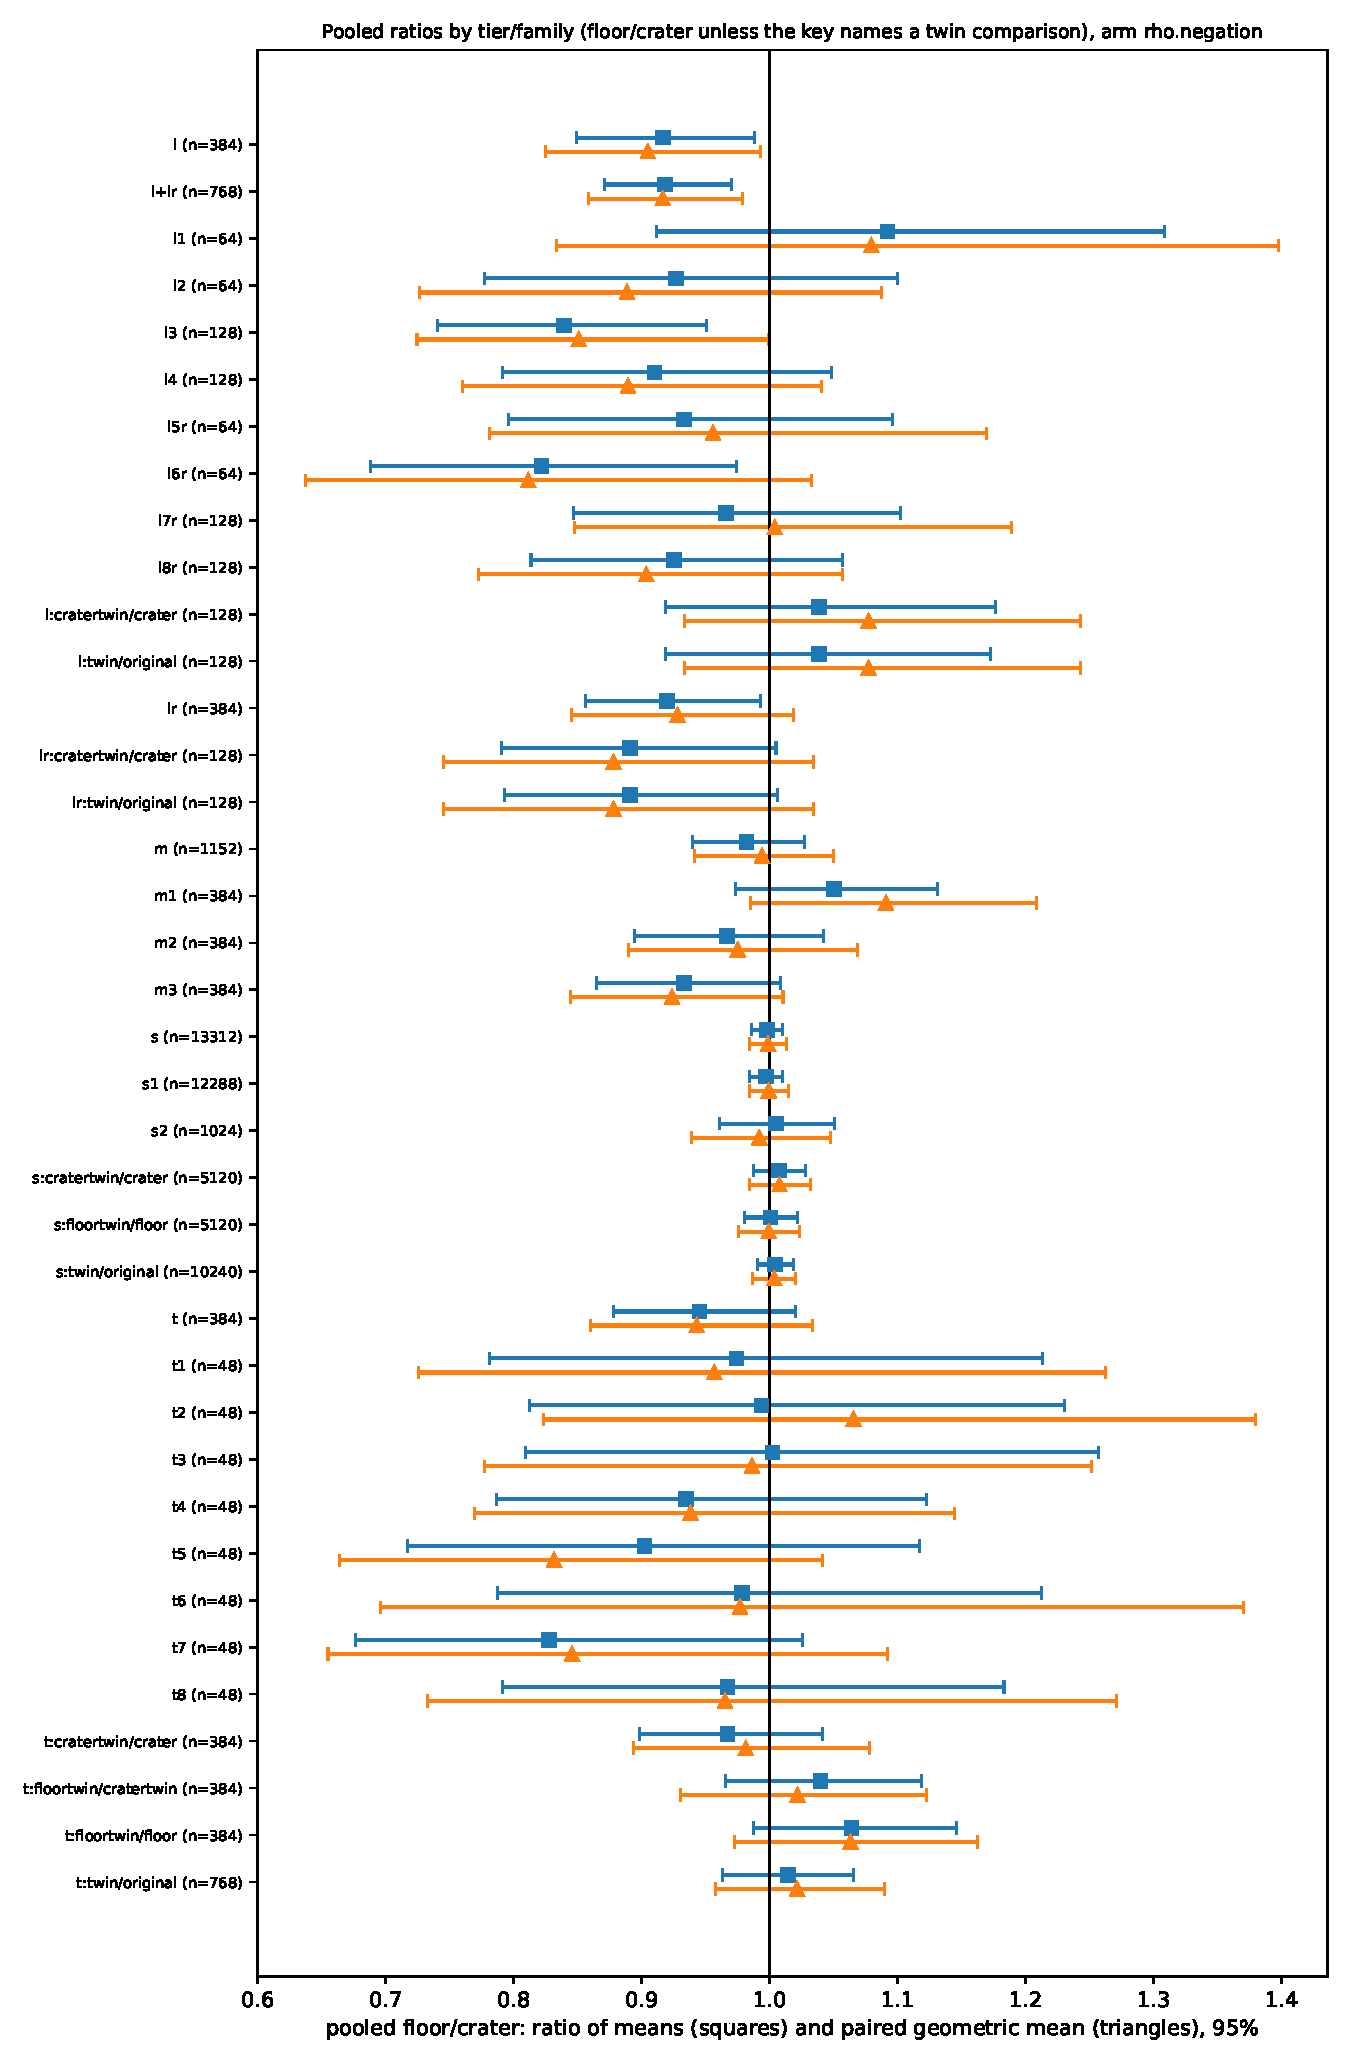
\includegraphics[width=0.92\textwidth]{figures/pooled_ratios.pdf}
\caption{Pooled ratios by tier and family, arm \texttt{rho.negation}:
ratio of means (squares, bootstrap 95\,\%) and paired geometric mean
(triangles). Keys without a colon are floor/crater; keys with a colon
are the named twin comparison. \texttt{s}: $\ell = 8209$ and $131101$;
\texttt{m}: $\ell \approx 2^{20}$; \texttt{l}, \texttt{lr}, \texttt{t}:
the frozen, replication and twin rounds at $\ell \approx 2^{25}$.
Source: \artefact{figures/pooled\_ratios.svg}, plotted from
\artefact{results/summary.json}.}
\label{fig:pooled}
\end{figure}

\begin{figure}[t]
\centering
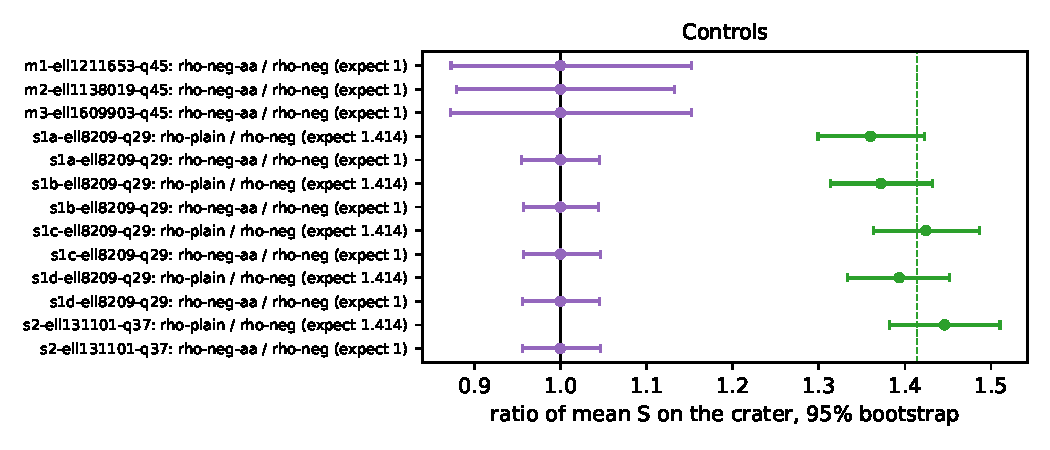
\includegraphics[width=0.8\textwidth]{figures/controls.pdf}
\caption{Controls on the crater of each tier S and M session: the
positive control \texttt{rho.plain}/\texttt{rho.negation} (expected
$\sqrt2$, dashed) and the A/A arm, which shares the algorithm seed with
the reference and therefore reproduces it exactly. Source:
\artefact{figures/controls.svg}.}
\label{fig:controls}
\end{figure}

\subsection{The easy gap: tier L and its follow-ups}

The frozen tier L (24 pairs at $\ell \approx 2^{25}$, 16 targets per
curve) pooled to $0.917\,[0.850, 0.988]$: the floors used fewer
operations than the craters, in the opposite direction to the companion
repository's earlier post-hoc value on the same pairs
($1.17\,[1.00, 1.38]$, one target each). The frozen rule did not reject
$H_0$: no single pair survived the Bonferroni correction (two of 24
excluded 1 on their own), and one of the eight twin controls in the tier
excluded 1 in the other direction ($1.59\,[1.20, 2.18]$). Two follow-ups
were then pre-registered and run on the same pairs with fresh target
seeds (Table~\ref{tab:L}).

\begin{table}[t]
\centering\footnotesize
\resizebox{\textwidth}{!}{%
\begin{tabular}{llcccc}
\toprule
round & design & floor / crater & crater-twin / crater & floor-twin / floor & floor-twin / crater-twin \\
\midrule
L frozen & 24 pairs, 8 crater twins ($u=3$) & $0.917\ [0.850, 0.988]$ & $1.039\ [0.919, 1.176]$ & & \\
replication & same curves, fresh targets & $0.920\ [0.856, 0.993]$ & $0.891\ [0.791, 1.005]$ & & \\
L $+$ replication & 48 pair-samples & $0.919\ [0.871, 0.970]$ & & & \\
twin round & twins of both ends ($u=5$) & $0.945\ [0.878, 1.021]$ & $0.967\ [0.898, 1.042]$ & $1.064\ [0.987, 1.146]$ & $\mathbf{1.040}\ [0.965, 1.119]$ \\
\bottomrule
\end{tabular}}
\caption{Tier L and its two pre-registered follow-ups, arm
\texttt{rho.negation}, ratio of means with bootstrap 95\,\% intervals,
$384$ solves per side in each pooled cell ($768$ for L $+$ replication).
Source: \artefact{results/summary.md}, pooled rows \texttt{l},
\texttt{lr}, \texttt{l+lr}, \texttt{t} and their twin keys.}
\label{tab:L}
\end{table}

The replication reproduced the frozen ratio almost exactly
($0.920$ against $0.917$), so the deficit is not a single unlucky draw;
over 48 pair-samples the floors cost $8\,\%\ [3\,\%, 13\,\%]$ fewer
operations than the craters. But the replication's twin control moved by
the same amount with no change of endomorphism ring
($0.891\,[0.791, 1.005]$), and the pairs whose intervals excluded 1 were
driven by high-$S$ crater draws that depressed the twin ratio of the
same pair just as much. The twin round was designed to separate the two
readings. Its three pre-registered comparisons all contain 1, and the
decisive one, floor-twin against crater-twin, is $1.040\,[0.965, 1.119]$:
the same conductor gap between two freshly re-coordinatised models shows
no deficit at all, while the comparisons involving the original crater
models ($0.945$, $0.967$) keep a few percent of it. The shift attaches to
the particular coordinate models of the pair file (all 24 craters are
the same $j_K$ model family, constructed the same way), not to $\End E$.
What remains is a statement about the harness's fixed partition hash: on
specific models it can move rho's mean cost by about five percent at
$n = 384$, which is exactly the residual that Section~\ref{sec:lean}
says a fixed hash can carry and that a uniformly random hash cannot.
The earlier post-hoc $1.17$ on these pairs is closed the same way.

\begin{figure}[t]
\centering
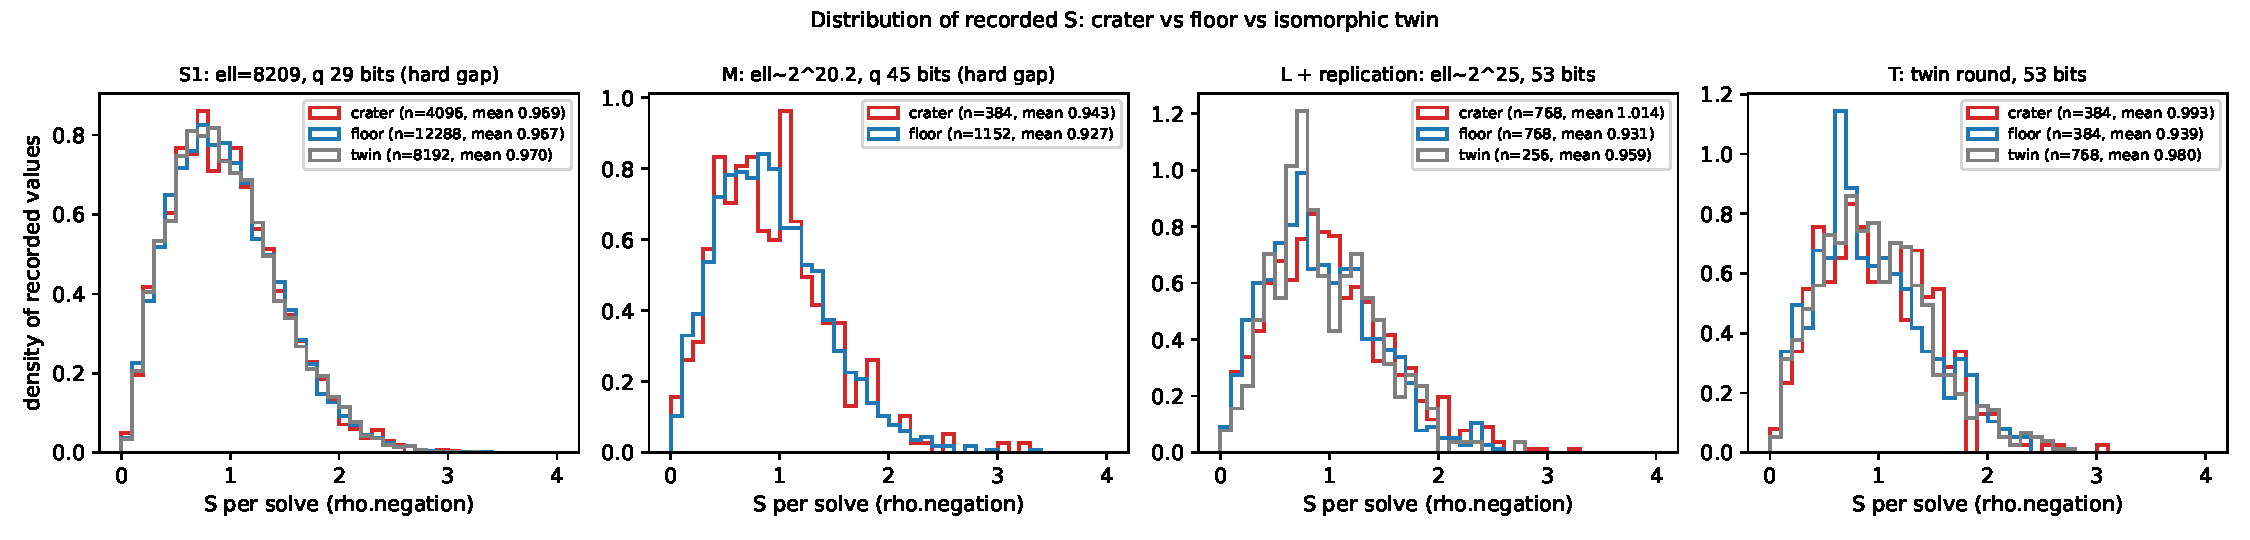
\includegraphics[width=\textwidth]{figures/s_distributions.pdf}
\caption{Distribution of recorded $S$ per solve, crater against floor
against isomorphic twin, in the $\ell = 8209$ shards, tier M, tier L with
its replication, and the twin round. Source:
\artefact{figures/s\_distributions.svg}, plotted from the session
records.}
\label{fig:dist}
\end{figure}

\section{A formal invariance for representation-hashing walks}
\label{sec:lean}

The generic-group argument~\cite{Nechaev1994,Shoup1997} says that an
algorithm whose control flow depends only on equality answers has the
same transcript on isomorphic groups; the companion repository had
already machine-checked this
(\artefact{crypto:research/conductor\_gap\_cm\_pairs\_20261010/lean/GenericInvariance.lean}),
and an integrity audit had pointed out that it does not cover the rho
and kangaroo the harness runs, because they hash the point representation.
We close that gap in the only form in which it is true: not for one fixed
hash, but for the space of hashes.

\begin{definition}
Let $G$ be a type with a binary operation $\cdot$ (no axioms are used).
An $r$-adding walk on $G$ is a pair $w = (h, m)$ with $h\colon G \to
\{0, \dots, r-1\}$ (the partition of the representation) and $m\colon
\{0, \dots, r-1\} \to G$ (the multipliers); its step is $x \mapsto x
\cdot m(h(x))$, its trajectory from $x$ of length $n$ is
$[x, \mathrm{step}\,x, \dots, \mathrm{step}^n x]$, and its
$\rho$-length with budget $B$, $\rho_w(x, B)$, is the least $n \le B$ whose
trajectory contains a repeated element, or $B + 1$ if none does.
Given a bijection $\varphi\colon G \to H$ with $\varphi(a \cdot b) =
\varphi a \cdot \varphi b$, the \emph{transport} of $w$ is the walk
$\varphi_* w = (h \circ \varphi^{-1},\ \varphi \circ m)$ on $H$.
\end{definition}

\begin{theorem}[\texttt{rhoCost\_transport}, \texttt{costPreservingBijection}]
\label{thm:transport}
For every walk $w$ on $G$, start $x \in G$ and budget $B$,
the trajectory of $\varphi_* w$ from $\varphi x$ is $\varphi$ applied
pointwise to the trajectory of $w$ from $x$, and
$\rho_{\varphi_* w}(\varphi x, B) = \rho_w(x, B)$. The map
$w \mapsto \varphi_* w$ is a bijection from the walks on $G$ to the walks
on $H$, with inverse $(\varphi^{-1})_*$.
\end{theorem}

\begin{proof}
One step commutes: $\varphi(x \cdot m(h x)) = \varphi x \cdot \varphi(m(h
x)) = \varphi x \cdot (\varphi \circ m)((h \circ \varphi^{-1})(\varphi
x))$. Induction gives the trajectory statement. A list has a repeated
element if and only if its image under an injective map does, and
$\varphi$ is injective, so the first index with a repeat is the same;
hence the $\rho$-lengths agree for every budget. The two transports
compose to the identity on both sides because $\varphi^{-1} \circ \varphi
= \mathrm{id}$ and $\varphi \circ \varphi^{-1} = \mathrm{id}$.
The formal proof
(\url{crypto:research/conductor_gap_rho_large_sample_20261018/lean/RepresentationHashInvariance.lean},
Lean 4.34.1, no dependencies) follows exactly these lines, with the
collision test written as a decidable Boolean on lists so that no
classical choice is needed; \texttt{\#print axioms} reports
\texttt{propext} and \texttt{Quot.sound} only (\artefact{lean/build.log}).
\end{proof}

\begin{remark}[What the theorem says about the conductor]
Two curves of the same prime order in one isogeny class have isomorphic
groups of points, so Theorem~\ref{thm:transport} applies with any
isomorphism $\varphi$ between them. Because the transport is a bijection
of the walk space, the push-forward of the uniform distribution on
$(h, m)$ is uniform: over a uniformly random partition and random
multipliers, the distribution of rho's $\rho$-length is identical on the
crater and on the floor. The endomorphism conductor, the $j$-invariant or
any other invariant that is not an invariant of the abstract group can
enter rho's cost only through the one fixed partition an implementation
uses. That residual is what Section~4 measures: at most about two percent
at $n = 1024$ on the twins, and about five percent on the specific
models of tier L.
\end{remark}

\begin{remark}[What the theorem does not say]
Nothing about curves, isogenies or endomorphism rings is formalised; the
bridge ``isogenous curves of equal prime order have isomorphic groups''
is an elementary fact used outside the file. The theorem is silent about
algorithms that are not walks of this shape, and about any fixed hash.
Together with the repository's transfer bound
(\artefact{TransferBound.lean}: any solver on one side yields a solver on
the other at the cost of two isogeny evaluations), the formal picture is:
generic algorithms are blind to the gap by theorem; representation-hashing
walks are blind in distribution by theorem and blind in practice by
measurement; any other algorithm can differ across the gap by at most the
cost of the connecting isogeny.
\end{remark}

\section{Discussion}

\paragraph{What is settled.}
For Pollard rho with the negation map, as implemented in a native,
audited harness, the floor and the crater of a prime conductor gap are
indistinguishable at the one-percent level for $\ell = 8209$ (29-bit
$q$), at the five-percent level for $\ell = 131101$ (37-bit) and at the
six-percent level for $\ell \approx 2^{20}$ (45-bit), all with a hard
kernel (field degree $2736$ to $\ell - 1$), under a fresh seed, with the
positive control confirming the detector and the twin controls bounding
the representation effect at the same level. The companion repository's
one open rho lead is closed, and so is its one post-hoc value at
$\ell \approx 2^{25}$, by attribution to the coordinate models.

\paragraph{Why the result is not surprising, and why it had to be measured.}
In the generic model the answer is forced by the group order; what is not
forced is the behaviour of a walk whose partition reads coordinates. The
twin controls quantify that non-generic residual directly, and the tier L
episode shows that it is real at the few-percent level for specific
models: the same deficit appeared twice under independent targets, and
only a design that re-coordinatised both endpoints could tell it apart
from a conductor effect. Earlier leads in both directions on the same
curves, with four and with one target per curve, were the same residual
seen through too few samples.

\paragraph{What is not settled.}
Whether some non-generic algorithm exploits $\End E = \ZZ + \ell\OK$
against $\OK$. The transfer bound says any such advantage is at most the
cost of one $\ell$-isogeny evaluation, which for a non-rational kernel
scales as $\ell^{2.6}$ in the repository's measurement; nobody has a
cheaper way, and nobody has proved there is none (computing the
endomorphism ring itself is subexponential~\cite{BissonSutherland2011},
but evaluating a specific vertical isogeny of large prime degree is not
known to be). A proof of equal hardness in the sense of the title
question would need lower bounds on the ECDLP that exist for no curve.
Index calculus is not measured here; the companion repository reports
$0.980\,[0.866, 1.111]$ for it at $\ell \approx 2^{25}$. Everything here
is over prime fields, $D_K = -19$, $q \le 53$ bits and one walk.

\paragraph{Classification.}
Under the companion repository's rules this is a null result on a
measured question, with one observation about the harness's partition
hash; it is not an advance, an engineering gain, a relabelling or an
accounting change, and it makes no security claim about any deployed
curve.

\section{Reproduction}

\artefact{make\_specs.py} writes the specifications; \artefact{run\_sessions.sh}
runs one harness session per specification; \artefact{audit.sh} produces
the receipts; \artefact{analyze.py} is the fixed analysis;
\artefact{plot.py}, \artefact{make\_run\_reports.py} and
\artefact{make\_report.py} lay out the recorded values. The 19 sessions of
tiers M, L and the follow-ups are committed raw; the five tier-S sessions
(420~MB) are committed as unmodified tarballs with checksums alongside
their full-replay receipts. Two harness pitfalls met on the way are
recorded with the amendments: an explicit CPU list made this build of the
harness exit without a session, and per-execution process overhead of
about $0.3$~s dominates small-field sessions.

\clearpage
\bibliographystyle{plain}
\bibliography{refs}

\end{document}
